%!TEX root = ../synopsis.tex

\section*{ОСНОВНОЕ СОДЕРЖАНИЕ РАБОТЫ}
Во {\bf введении}
обосновывается актуальность диссертационной работы,
определены цель и задачи исследования,
представлена научная новизна, теоретическая и практическая значимость работы.
Приведены основания для выполнения работы, ее апробация и структура.


%!TEX root = ../synopsis.tex

В {\bf первой главе}
проводится анализ проблемы автоматизированного проектирования УП
в раскройно-заготовительном производстве для оборудования термической фигурной резки с ЧПУ.
Описаны основные технологические особенности и ограничения термической резки,
которые необходимо соблюдать при проектировании УП.

\begin{figure}[h]
  \centering
  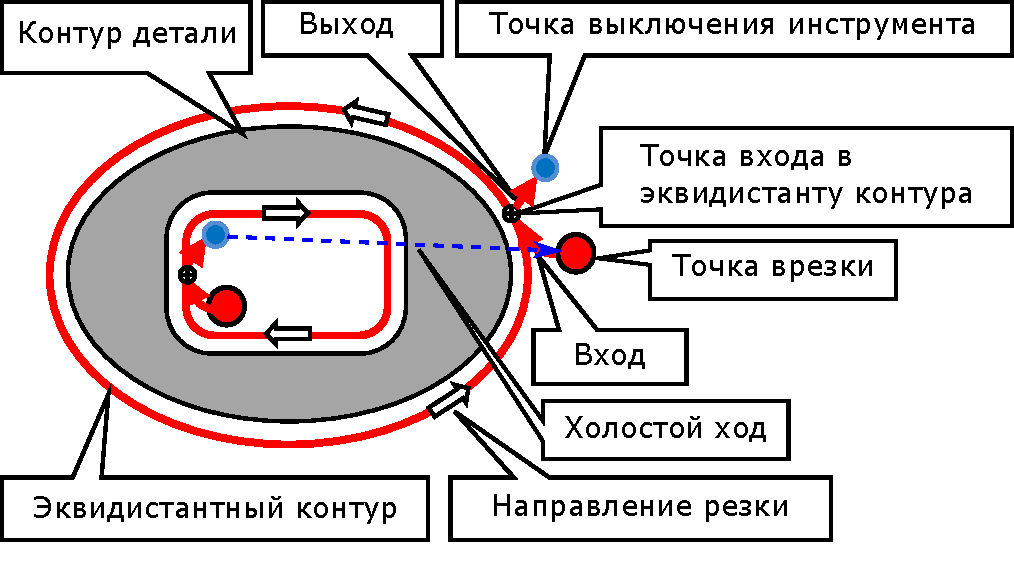
\includegraphics[width=0.8\textwidth]{toolpath.pdf}
  \caption{Элементы маршрута резки}
  \label{fig:toolpath}
\end{figure}

В общем случае маршрут инструмента содержит несколько компонент:
начальную $M_0$
и возможно отличную от неё конечную точку маршрута $M_{N+1}$,
$N$~точек врезки $M_i$, $i \in \overline{1, N}$
и соответствующих им точек выключения инструмента
$M_i^*$,
рабочий ход инструмента от точки врезки $M_i$
до точки выключения $M_i^*$
(в дальнейшем будем называть его траекторию
{\it сегментом резки}
$S_i=M_i M_i^*$)
а также холостой ход от $M_i^*$
до следующей точки врезки $M_{i+1}$,
см.~рис.~\ref{fig:toolpath}.
В определение маршрута также входит
порядок резки,
то есть последовательность посещения точек врезки,
представляющая собой перестановку
$I = (i_1, i_2, ... i_N)$.
Таким образом,
маршрут резки можно определить
в терминах сегментов резки как кортеж
\begin{equation}
  \mathfrak{R} = \left<
    M_0, M_1, S_1, M_1^*, M_2, S_2, M_2^*, \,\dots, M_N, S_N, M_N^*,
    i_1, i_2, \,\dots, i_N
  \right>
  \label{eq:route:tuple}
\end{equation}

В качестве целевой функции при оптимизации часто используется время резки
\begin{equation}
  T_{cut} = \frac{L_{on}}{V_{on}} + \frac{L_{off}}{V_{off}} +N_{pt} \cdot t_{pt}
  ,
  \label{eq:cutting-time}
\end{equation}
где
$L_{on}$ -- длина реза с включенным режущим инструментом;
$V_{on}$ -- скорость рабочего хода режущего инструмента;
$L_{off}$ -- длина переходов с выключенным режущим инструментом (холостой ход);
$V_{off}$ -- скорость холостого хода;
$N_{pt}$ -- количество точек врезки;
$t_{pt}$ -- время, затрачиваемое на одну врезку.
В подавляющем большинстве исследований,
включая данную диссертационную работу,
$V_{on}$ считается константой
(в рамках конкретной УП),
однако вообще говоря это не так,
см.~\cite{Obuhovo}.

Важнейшей экономической характеристикой качества
разработанной управляющей программы является стоимость
(себестоимость) резки деталей на машине с ЧПУ.
По аналогии с \eqref{eq:cutting-time}
его можно определить по формуле
\begin{equation}
  F_{cost}=
  L_{on} \cdot C_{on} +
  L_{off} \cdot C_{off} +
  N_{pt} \cdot C_{pt}
  ,
  \label{eq:cutting-cost}
\end{equation}
где
$C_{on}$ -- стоимость единицы пути с включенным режущим инструментом;
$C_{off}$ -- стоимость единицы пути с выключенным режущим инструментом;
$C_{pt}$ -- стоимость одной врезки.

Задача оптимизации маршрута инструмента для машин фигурной листовой резки с~ЧПУ
может быть представлена в общем виде
как задача минимизации некоторой числовой функции
$\mathfrak F$
(например, \eqref{eq:cutting-time} или \eqref{eq:cutting-cost})
на множестве
$\mathfrak G$ допустимых кортежей
\eqref{eq:route:tuple}:
\begin{equation}
  \mathfrak F(\mathfrak R) \to \min_{\mathfrak R \in \mathfrak G}
  \label{eq:cut:problem}
\end{equation}

В маршрут \eqref{eq:route:tuple} помимо перестановки
$I = (i_1, i_2, ... i_N)$
входят также точки $M_i$ и $M_i^*$,
которые в общем случае должны ещё быть выбраны
из некоторого непрерывного множества,
что делает простую формулировку задачи \eqref{eq:cut:problem}
чрезвычайно сложной в решении.
Более того,
набор сегментов резки $S_i$
в общем случае не совпадает
(даже в количестве)
с набором контуров деталей,
подлежащих резке,
так как на практике используются различные техники резки:
\begin{enumerate}
  \item
  {\it Резка по замкнутому контуру (стандартная техника)}:
  сегмент резки содержит
  ровно один замкнутый контур заготовки
  и вырезается целиком.
  \item
  {\it Мультисегментная резка}:
  для вырезки одного контура
  используются не менее двух сегментов резки.
  \item
  {\it Мультиконтурная резка}:
  резка предполагает вырезку нескольких
  контуров в одном сегменте.
\end{enumerate}

В зависимости от используемой техники резки и
способа выбора точек врезки можно выделить
несколько классов задач резки
\autocite[]{bi:dewil-review},
изображенных на рис.~\ref{fig:cut-classes}:

\begin{figure}
  \centering
  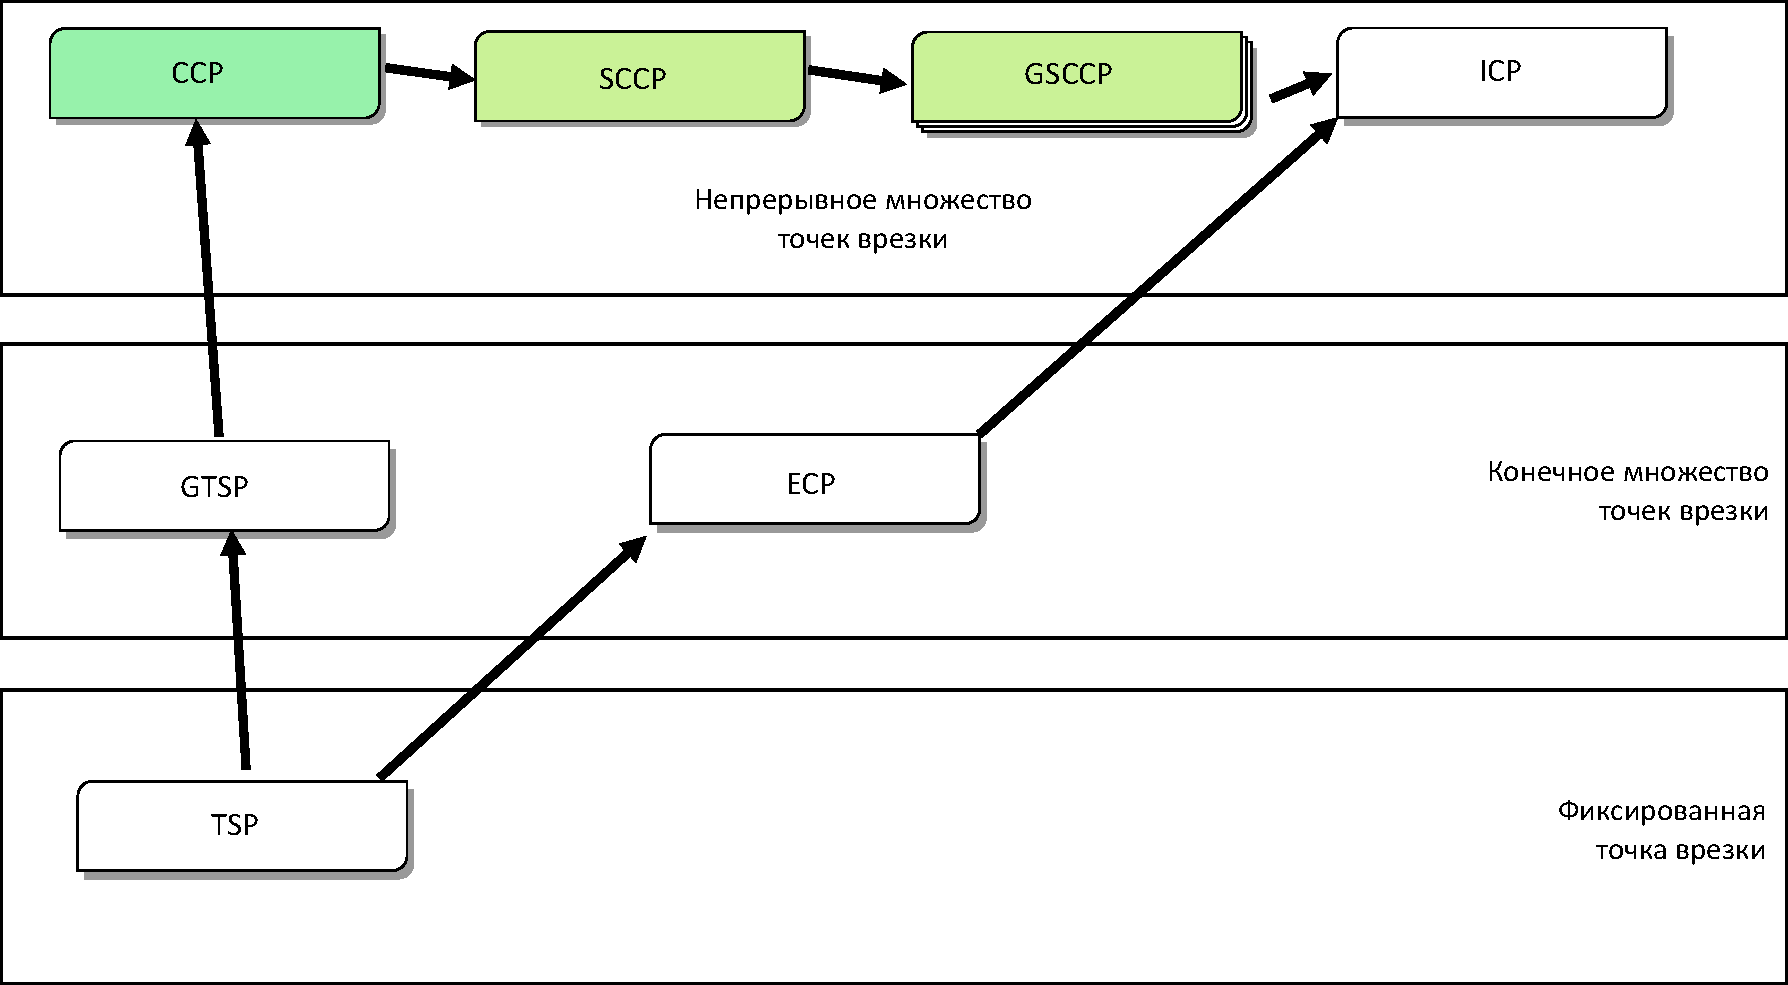
\includegraphics[width=0.95\textwidth]{classes.pdf}
  \caption{Классификация задач резки}
  \label{fig:cut-classes}
\end{figure}

\begin{itemize}
  \item
  \textbf{Задача непрерывной резки}
  (Continuous Cutting Problem, CCP):
  каждый контур
  вырезается за один раз,
  одним движением инструмента,
  но резка может начаться в любой точке контура
  (и заканчивается в ней же)

  \item
  \textbf{Обобщённая задача коммивояжера}
  (Generalized Traveling Salesman Problem, GTSP):
  резка может начаться в одной из заранее
  заданных точек на контуре
  (количество таких точек конечно),
  после этого контур вырезается целиком

  \item
  \textbf{Задача резки с остановками}
  (Endpoint Cutting Problem, ECP):
  резка контура может начинаться только в
  заранее заданных точках на нём,
  но контур может вырезаться за несколько раз,
  частями

  \item
  \textbf{Сегментная задача непрерывной резки}
  (Segment Continuous Cutting Problem, SCCP):
  сегмент резки может быть частью контура
  или объединением нескольких контуров
  и / или их частей.
  Каждый сегмент вырезается целиком,
  от начала до конца,
  таким образом
  $ CCP \subset SCCP$.

  \item
  \textbf{Обобщённая сегментная задача непрерывной резки}
  (Generalized Segment Continuous Cutting Problem, GSCCP):
  подобна сегментной задаче непрерывной резки
  (SCCP),
  но разбивка на сегменты не задана заранее
  и сама подлежит оптимизации

  \item
  \textbf{Задача прерывистой резки}
  (Intermittent Cutting Problem, ICP):
  наиболее общая формулировка задачи резки,
  встречающаяся в научной литературе,
  контуры могут вырезаться частями,
  в несколько подходов,
  начиная с произвольной точки.
\end{itemize}

На практике
задача маршрутизации режущего инструмента
чаще всего решается
как задача дискретной оптимизации,
для этого непрерывный контур детали
заменяется на конечное число
потенциальных точек врезки,
как правило расположенных на нём
с некоторым шагом
$\varepsilon$,
то есть фактически сводится к
ECP
или её частному случаю --
GTSP.

Полученный любым способом
маршрут движения режущего инструмента,
должен быть исполнен
на конкретном промышленном оборудовании --
режущей машине с ЧПУ.
Это накладывает ряд
существенных ограничений
на решение задачи резки,
то есть ограничивает множество
$\mathfrak G$ в \eqref{eq:cut:problem}.

Наиболее популярным и хорошо описанным в литературе
является так называемое
{\it ограничение предшествования}
(Precedence Constraint, PC),
возникающее из-за того,
что
после вырезания замкнутого контура,
его внутренняя часть ничем не удерживается
и может сдвигаться, поворачиваться, наклоняться
или даже падать.
Поэтому внутренние отверстия деталей следует
вырезать до того,
как будет завершена резка
внешнего контура детали.
Аналогично,
если меньшая деталь размещается
(в целях экономии расхода материала)
в отверстии большей детали,
она должна целиком быть вырезана
до того,
как будет завершена резка
содержащего её отверстия
и тем более --
внешнего контура большей детали.
В терминах маршрута~\eqref{eq:route:tuple}
не все перестановки
$I = (i_1, i_2, ... i_N)$
оказываются допустимы.

Большинство технологий резки
(например, лазерная, газовая или плазменная)
требуют,
чтобы резак двигался не строго по контуру детали,
а с некоторым припуском,
так как часть материала повреждается в процессе резки.
Введение этого припуска может происходить
на разных этапах технологической подготовки производства --
при решении задачи резки;
при генерации управляющей программы для станка с ЧПУ;
самим станком ЧПУ прямо в процессе резки.
Точка врезки в контур
(включения резака)
должна располагаться
как правило ещё на большем расстоянии
от контура детали
во избежание её повреждения.
В данной диссертационной работе,
однако,
эти ограничения не рассматриваются,
то есть
далее везде предполагается,
что режущий инструмент движется точно по контуру детали
и точка врезки
(которая в данном случае
является и точкой выключения инструмента
после окончания вырезания контура)
всегда расположена точно на контуре.

В литературе описан
ещё целый ряд ограничений,
накладываемых на маршрут режущего инструмента,
порождаемых
технологическими свойствами
современных машин термической резки с ЧПУ,
которые также должны учитываться
при практическом применении,
см. в частности
\cite{Sozopol,Miskolc}.
В данной диссертационной работе
эти технологические ограничения также не рассматриваются.

%!TEX root = ../synopsis.tex

Во {\bf второй главе}
рассматривается задача непрерывной резки {\it CCP}
на Евклидовой плоскости
$\mathbb R \times \mathbb R$.
Возьмём
$N$
попарно непересекающихся плоских контуров
$\{C_1, C_2, ... C_N\}$,
ограничивающих
$n$
деталей
$\{A_1, A_2, ... A_n\}$.
В общем случае
$n \leqslant N$.
В данной работе рассматриваются только контуры
$C_i$,
состоящие из
(конечного числа)
отрезков прямых линий и дуг окружностей,
так как именно такие геометрические примитивы
поддерживаются программным обеспечением
современных машин термической резки с ЧПУ.
Выберем также две точки
$M_0$, $M_{N + 1}$
(почти всегда $M_0 = M_{N + 1}$),
которые будут использоваться
как начало и конец
маршрута резки.
Задача непрерывной резки
({\it Continuous Cutting Problem, CCP})
состоит в поиске:
\begin{enumerate}
\item
$N$ точек врезки $M_i \in C_i, i \in \overline{1, N}$
\item
Последовательности обхода контуров
$C_i$,
то есть перестановки
$N$
элементов
$I = (i_1, i_2, ... i_N)$
\end{enumerate}
Результатом решения задачи будет являться маршрут
\begin{equation}
  \label{eq:route}
  \mathcal R =
  \left<M_0, M_{i_1}, M_{i_2}, \dots M_{i_N}, M_{N + 1}\right>
\end{equation}
Целевая функция
сводится фактически к минимизации длины холостого хода:
\begin{equation}
  \mathcal{L} = \sum_{j=0}^N|M_{i_j}M_{i_{j+1}}|
  \label{air-move-length}
\end{equation}
$$
\mathcal{L} \to \min
$$
где, для простоты записи мы полагаем
$M_{i_0} = M_0$,
$M_{i_{N + 1}} = M_{N + 1}$.

Кроме того, решение должно удовлетворять ограничению предшествования:
если
$\widetilde C_i$
обозначает 2-мерную фигуру,
ограниченную контуром
$C_i$
(в более традиционных обозначениях
$C_i = \partial \widetilde C_i$),
то
$
 \widetilde C_p \subset \widetilde C_q \Rightarrow i_p < i_q
$,
то есть вложенный контур должен быть посещён раньше,
чем содержащий его,
и не все перестановки
$I = (i_1, i_2, ... i_N)$
допустимы.

Предлагаемый алгоритм
(см.~\cite{berlin2019,bi:ccp:ru})
решения задачи:

\begin{enumerate}
  \item Удаление <<внешних>> контуров
  \item Поиск положений точек врезки (непрерывная оптимизация)
  \item Поиск порядка обхода контуров (дискретная оптимизация без учёта ограничений предшествования)
  \item Восстановление удалённых контуров
\end{enumerate}

На первом шаге мы удаляем все контура,
внутри которых содержатся другие,
то есть оставляем только
$$
\{C_i | \forall j \ne i: C_j \cap \widetilde C_i = \varnothing \},
$$
тем самым как правило сокращая размерность задачи с $N$
до некоторого $N' \leqslant N$.

На втором шаге мы предполагаем перестановку контуров
$I = (i_1, i_2, ... i_N)$
фиксированной,
выбираем произвольные положения точек врезки
$M_i \in C_i$ на контурах и подвергаем их последовательной релаксации:
для каждой точки $M_i$
мы полагаем все остальные $M_j$ $(i\ne j)$ фиксированными и находим
положение $M_i$, минимизирующее функционал
$$
|M_{i-1}M_i|+|M_iM_{i+1}| \to \min_{M_i \in C_i}
$$

На практике этот процесс очень быстро сходится,
получая за время $O(N')$
позиции точек врезки на всех контурах.

На третьем шаге предполагается воспользоваться каким-либо
методом дискретной оптимизации для поиска перестановки
$I = (i_1, i_2, ... i_N)$.
В данной диссертационной работе использован метод
переменных окрестностей
(Variable Neighborhood Search,
VNS
\autocite{bi:VNS}).
Мы также начинаем с произвольной
(случайной перестановки $I$),
строим окрестность этой перестановки
$\mathcal N(I)$
(например, все перестановки,
полученные из неё всеми однократными попарными перестановками контуров),
для каждой перестановки $I'\in \mathcal N(I)$
находим оптимальные позиции точек врезки
для минимизации холостого хода
$$
\mathcal L (I') = \min_{M_1, M_2 \dots M_N}
  \mathcal L (M_1, M_2 \dots M_N | I')
$$
(как описано выше на втором шаге алгоритма)
и выбираем ту из перестановок $I'$,
которая даёт наименьшее значение длины
холостого хода \eqref{air-move-length},
и к ней применяется этот же процесс.
Если же понизить длину холостого хода не получается,
рассматриваются всё более широкие окрестности
$\mathcal N(I)$
(например, полученные тройными перестановками контуров
и т.п.),
пока не будет обнаружена перестановка $I$,
которая уже не может быть улучшена.
Она и считается решением задачи
вместе с соответствующими ей позициями точек врезки.

На четвёртом и последнем шаге алгоритма
мы восстанавливаем контуры,
удалённые на первом шаге и находим точки
врезки и для них как пересечение маршрута
\begin{equation}
  \label{eq:route0}
  \mathcal R = \left< M_0, M_1, M_2, \dots M_{N'}, M_{N+1}\right>
\end{equation}
с каждым из (удалённых) контуров
$M_i = C_i \cap \mathcal R$,
причём из нескольких таких точек
выбирается самая последняя по ходу маршрута
\eqref{eq:route0}.
После добавления таким образом всех
<<внешних>> контуров
и соответствующих им точек врезки,
мы получаем уже полный маршрут,
который посещает все исходные контуры,
причём внутренние контуры посещаются
строго раньше содержащих их внешних.
Полная длина маршрута
при этой операции,
очевидно,
не меняется.
Получаемый таким образом полный маршрут
является оптимальным решением исходной задачи
непрерывной резки,
при этом
мы строго выполняем
ограничение предшествования,
тратя на это линейное время
$O(N)$.

Как для любой эвристики,
возникает вопрос оценки качества решения,
получаемого данным алгоритмом.
Действительно, легко построить пример,
см. рис.~\ref{fig:counter-example},
когда
(даже для фиксированного порядка посещения контуров),
может быть получено два маршрута резки,
в зависимости от начальных точек врезки.

\begin{figure}
  \begin{center}
  \begin{tikzpicture}[scale=2.7]
    \draw
      (1,-0.2) node(M3){} circle(0.027) node[below] {$M_3$}
      (-1,-0.2) node(M0){} circle(0.027) node[below] {$M_0$};
    \draw [thick,pattern=north west lines]
      (1.3,0) -- (2,0) -- (2,1) node[midway,left]{$C_2$} -- (1,1) node(M2x){} --
      (1, 1.1) -- (2.1,1.1) -- (2.1,-0.1) -- (1.3, -0.1) node(M2) {} --cycle
    % \draw [thick,pattern=north west lines]
      (-1.3,0) -- (-2,0) -- (-2,1) node[midway,right]{$C_1$} -- (-1,1) node(M1x){} --
      (-1, 1.1) -- (-2.1,1.1) -- (-2.1,-0.1) -- (-1.3, -0.1) node(M1){} --cycle;
    \draw[dashed]
      (M0) -- (M1) -- (M2) node[midway,above]{Глобальный минимум} -- (M3);
    \draw[dashed]
      (M0) -- (M1x) -- (M2x) node[midway,below]{Локальный минимум} -- (M3);
  \end{tikzpicture}
  \end{center}
  \caption{Два маршрута резки для одной задачи CCP  }
  \label{fig:counter-example}
\end{figure}

В ходе данной диссертационной работы были доказаны несколько свойств получаемого маршрута
в предположении, что все контуры являются многоугольниками:

\begin{itemize}
  \item
  {\it Локальный минимум}:
  сдвиг нескольких соседних точек врезки на маршруте \eqref{eq:route}
  в пределах {\bf тех же самых} сегментов контуров,
  на которых они расположены,
  не приводит к уменьшению полной длины маршрута \eqref{air-move-length}.
  \item
  {\it Глобальный минимум}.
  сдвиг нескольких соседних точек врезки на маршруте \eqref{eq:route}
  в пределах содержащих их контуров
  не приводит к уменьшению полной длины маршрута \eqref{air-move-length},
  если для каждой  точки врезки $M_i \in C_i$ выполнено одно из условий:
  \begin{enumerate}
    \item
    Сегмент
    $M_{i-1} M_{i+1}$
    пересекает контур
    $C_i$,
    то есть
    $M_i \in M_{i-1} M_{i+1}$
    \item
    Касательная в точке
    $M_i$
    к эллипсу с фокусами
    $M_{i-1}$
    и
    $M_{i+1}$
    и проходящему через
    $M_i$,
    разделяет эллипс и контур
    $C_i$

    Это условие легко проверяется программно,
    однако можно выделить несколько практически полезных частных случаев,
    когда оно проверяется просто визуально:
    \begin{itemize}
      \item
      Вершина
      $M_i$
      является внутренней точкой одного из
      отрезков контура
      $C_i$
      и при этом весь контур расположен
      по одну сторону линии,
      проходящей через этот отрезок
      \item
      Вершина
      $M_i$
      является также вершиной контура
      $C_i$
      (принадлежит сразу двум его отрезкам)
      и при этом весь контур находится
      внутри угла,
      образованного лучами,
      идущими из вершины
      $M_i$
      вдоль этих двух отрезков
      \item
      Контур
      $C_i$
      ограничивает собой выпуклый
      многоугольник
      $\widetilde C_i$.
    \end{itemize}
  \end{enumerate}
\end{itemize}

С практической точки зрения
алгоритм работает очень хорошо,
быстро находя хорошие маршруты резки.
Однако, объективная оценка качества решения сложна.
В данной работе в качестве базы сравнения использовался алгоритм
на основе динамического программирования
\autocite{bi:RoMa},
который находит точное решение задачи GTSP
для количества контуров
$N \leqslant 33$.
Использовались несколько раскройных планов,
содержащих реальные детали,
см. табл.~\ref{tab:ccp-vs-gtsp}.

\begin{table}[h!]
  \centering
  \caption{Сравнение качества решений задач CCP и GTSP}
  \label{tab:ccp-vs-gtsp}
  \def\arraystretch{1.2}
  \begin{tabular}{l|*{3}{r}}
      Задание & № 229 & № 464 & № 3211 \\
      \hline
      Кол-во деталей & 11 & 14 & 17\\
      Кол-во контуров & 12 & 21 & 22 \\
      Общий периметр, м & 24.609 & 21.717 & 25.051 \\
      Кол-во точек GTSP & 491 & 429 & 493 \\
      $\mathcal L_{GTSP}$, м & 7.729 & 4.743 & 4.557 \\
      $\mathcal L_{CCP}$, м & 7.727 & 4.706 & 4.536 \\
      \hline
  \end{tabular}
\end{table}

\begin{figure}[p]
  \begin{center}
    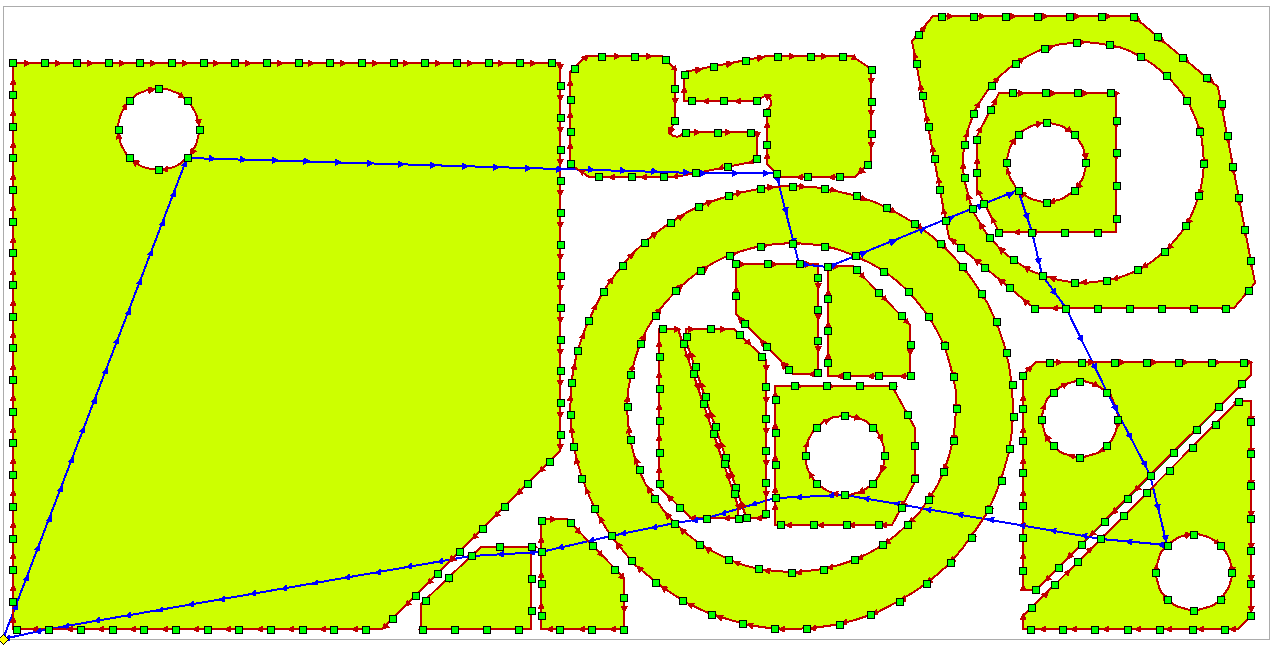
\includegraphics[width=0.95\textwidth]{464-gtsp.png}
  \end{center}
  \caption{Точное решение задачи GTSP для задания № 464}
  \label{fig:gtsp-path}
\end{figure}

\begin{figure}[p]
  \begin{center}
    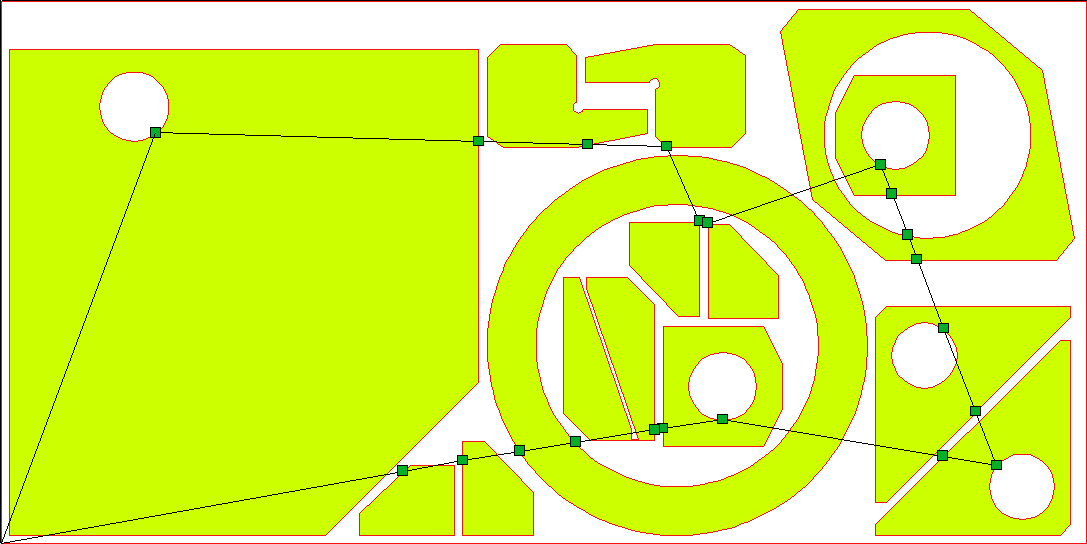
\includegraphics[width=0.95\textwidth]{464-ccp.png}
  \end{center}
  \caption{Решение задачи непрерывной резки для задания № 464}
  \label{fig:ccp-path}
\end{figure}

На рис. \ref{fig:gtsp-path}
показано точное решение задачи GTSP.
Хорошо видны возможные положения точек врезки,
которые получены путём дискретизации контура,
то есть сведения задачи непрерывной оптимизации
к задаче дискретной оптимизации.
На рис. \ref{fig:ccp-path}
показано решение задачи непрерывной резки,
полученное вышеописанным алгоритмом
для того же раскройного плана.

Видно,
что оба алгоритма дают практически идентичные
маршруты резки.
Основное отличие вызвано необходимостью дискретизации
контуров в ходе сведения задачи
непрерывной резки к GTSP.
Это приводит, в частности к тому,
что длина холостого хода в задаче GTSP
получается немного больше,
чем в задаче CCP,
что видно в табл.~\ref{tab:ccp-vs-gtsp}.

%!TEX root = ../synopsis.tex

В {\bf третьей главе}
рассматривается обобщённая задача коммивояжера с
ограничениями предшествования ({\it PCGTSP}) --
это хорошо известная задача комбинаторной оптимизации,
имеющая множество приложений помимо
оптимизации траектории режущего инструмента
и привлекшая внимание многих исследователей.
К сожалению,
в отличие от задачи GTSP,
алгоритмические подходы к решению
именно PCGTSP всё ещё малочисленны.
Алгоритм, предложенный в данной диссертационной работе,
на основе синтеза нескольких идей других исследователей,
представляет собой попытку
создать первый точный алгоритм
ветвей и границ для
решения задачи PCGTSP в общем виде.

Задача определяется тройкой
$(G,\mathcal C,\Pi)$,
где
$G=(V,E,c)$ -- взвешенный ориентированный граф на $n$
вершинах,
задающий веса $c(u,v)$ для всех своих ребер
$(u,v)\in E, u, v \in V$;
$\mathcal C=\{V_1,\ldots,V_m\}$ -- разбиение вершин
графа $G$ на $m$ кластеров;
$ \Pi = (\mathcal C, A) $ -- частичный порядок,
заданный на множестве кластеров.
Для каждой вершины
$v\in V$, за $V(v)$
обозначим (единственный) кластер
$V_p\in\mathcal C$,
такой что
$v\in V_p$.

Допустимым решением задачи
$(G,\mathcal C,\Pi)$
называется тур (замкнутый путь) $T$,
удовлетворяющий условиям:
\begin{itemize}
    \item
    имеет длину $|T|=m$
    \item
    начинается и заканчивается в некоторой вершине $v_1\in V_1$
    \item
    посещает каждый кластер $V_p\in\mathcal C$
    \item
	каждое ребро
	$(v_i, v_j)$ в $T$
	(кроме ребра $(v_m,v_1)$)
	удовлетворяет ограничению предшествования,
	то есть
	 $(V(v_i),V(v_j))\in A$.
\end{itemize}

Каждому решению
$T=v_1, v_2, \ldots, v_m$
мы назначаем стоимость
\begin{equation}
    \label{eq:pctgsp-cost}
	cost(T) = c(v_m,v_1) + \sum_{i=1}^{m-1} c(v_i,v_{i+1})
\end{equation}

Требуется найти допустимый тур
$ T $
с минимальной стоимостью
$$
cost (T) \to \min_T
$$

Ключевой идеей алгоритма является построение нижней оценки стоимости решения.
Для этого в каждой вершине дерева поиска исходная задача разделяется на две:
\begin{enumerate}
    \item
    Фиксируется {\it префикс}
    маршрута $\sigma=\{V_1, \dots, V_r\}$.
    Обозначим $c_{min}$ нижнюю границу длины
    всех путей, проходящих из вершин кластера $V_1$
    в вершины кластера $V_r$ строго в порядке $\sigma$.
    \item
    Построим вспомогательную задачу $\mathcal P$,
    удалив из исходной задачи все кластеры,
    являющиеся внутренними в $\sigma$ и
    соединив все вершины из $V_1$ с вершинами $V_r$
    ребрами нулевого веса.
    Полученная таким образом задача всё ещё сложна,
    однако она может быть несколькими способами
    упрощена (релаксирована) $\mathcal P \to \mathcal P_{rel}$
    и для неё найдено оптимальное решение $\mathrm{OPT}(\mathcal P_{rel})$
\end{enumerate}
Нижняя оценка $LB$
находится как
\begin{equation}
    \label{eq:pcgtsp-lb}
    LB = c_{\min} + \mathrm{OPT}(\mathcal P_{rel})
\end{equation}

В качестве релаксации $\mathcal P_{rel}$ задачи $\mathcal P$
могут применяться
\autocite[]{SALMAN2020163}:
\begin{itemize}
    \item
    хорошо известная трансформация Noon-Bean,
    преобразующая задачу GTSP в обычную задачу
    коммивояжера TSP
    \item
    построение вспомогательного {\it графа кластеров} $H_1$
    с весами, индуцированными весами исходного графа $G$:
    $$
    c(V_i, V_j) = \min_{v_i \in V_i, v_j \in V_j} c(v_i, v_j)
    $$
    \item
    построение графа кластеров $H_2$,
    веса в котором также индуцированы весами путей длины 2 в исходном графе $G$:
    $$
    c(V_i, V_j) =
        \min_{\substack{v_i \in V_i, v_j \in V_j\\v_k \notin V_i \cup V_j}  }
        \frac{c(v_i, v_k) + c(v_k, v_j)}{2}
    $$
    при этом маршрут $v_i, v_k, v_j$ должен удовлетворять ограничению предшествования $\Pi$.
    Этот способ позволяет точнее учитывать взаимное расположение контуров на плоскости
    в случае Евклидовой задачи PCGTSP
    \item
    по аналогии с $H_2$ могут строиться кластерные графы с весами на основе
    путей большей ($\geqslant 3$) длины,
    однако алгоритм их расчёта существенно сложнее и
    не входит в рамки данной диссертационной работы
\end{itemize}

Наконец, для (быстрого) поиска
нижней оценки на решение задачи $TSP(\mathcal P_{rel})$
можно использовать:
\begin{itemize}
    \item
    Решение задачи о минимальном остовном дереве
    (Minimal Spanning Arborescence, MSAP),
    так как $MSAP(\mathcal P) \leqslant TSP(\mathcal P)$
    \item
    Решение задачи о цикловом покрытии (Cycle cover);
    оно находится как решение задачи о назначениях
    (Assignment Problem, AP)
    для двудольного графа,
    обе доли которого представляют $\mathcal P_{rel}$;
    опять $AP(\mathcal P) \leqslant TSP(\mathcal P)$
    \item
    в некоторых случаях можно прямо решить задачу
    коммивояжера $TSP(\mathcal P)$.
    В данной работе для этого использовался решатель Gurobi
    и MIP-модель ATSPxy
    \autocite{SARIN2005}.
\end{itemize}

Все возможные методы оценки нижней границы показаны в табл.~\ref{t:LBs},
используемые в описываемой реализации обозначены
$L_1$--$L_3$,
не используемые --
$E_1$--$E_6$.
Проведённые численные эксперименты показывают,
что часть методов
($E_1$--$E_4$)
систематически дают более слабые оценки,
а часть
($E_1$--$E_2$, $E_5$--$E_6$)
требуют значительных временных затрат по сравнению с выбранными.
Оценка $L_3$
в этом смысле является компромиссом,
причём она вычисляется только для малой доли
префиксов
($\approx 1\%$)
с наименьшей оценкой, полученной методами
$L_1$--$L_2$.

\begin{table}
    \centering
    \caption{Методы оценки нижней границы}\label{t:LBs}
    \begin{tabular}[t]{*{5}{|c}|}
        \hline
        & \textbf{Noon-Bean} & $\mathbf{H_1}$ & $\mathbf{H_2}$ & $\mathbf{H_{3+}}$\\
        \hline \hline
      \textbf{AP} & $E_1$ & $\mathbf{L_1}$ & $\mathbf{L_2}$ & - \\
      \textbf{MSAP} & $E_2$ & $E_3$ & $E_4$ & - \\
      \textbf{Gurobi} & $E_5$ & $\mathbf{L_3}$ & $E_6$ & -\\
      \hline
    \end{tabular}
\end{table}

Получив описанными методами оценку нижней границы для данного префикса по формуле~\eqref{eq:pcgtsp-lb},
алгоритм принимает решение об отсечении ветви,
порождаемой текущим префиксом $\sigma$, при условии
\begin{equation}
    \label{eq:pcgtsp:cut}
    LB > UB,
\end{equation}
где $UB$ -- стоимость наилучшего известного допустимого решения исходной задачи.
В данной работе для получения $UB$
используется эвристика PCGLNS
\autocite{KKP-optima2020},
позволяющая буквально за несколько секунд получить
близкое к оптимальному решение исходной задачи PCGTSP,
что резко сокращает перебор,
позволяя отбрасывать $\approx 50\%$--$90\%$
ветвей.

Предлагаемый алгоритм ветвей и границ обходит дерево поиска,
начиная с корня
$\sigma=\{V_1\}$
в ширину
({\it Breadth-first search}),
для каждого узла
находя оценку нижней границы~\eqref{eq:pcgtsp-lb},
проверяя условие отсечения~\eqref{eq:pcgtsp:cut}
и для <<выживших>> узлов применяя процедуру ветвления.
Для этого он находит все кластера,
которые можно добавить в конец текущему префиксу,
не нарушая ограничение предшествования $\Pi$.
По окончании подсчёта префиксов одной длины,
алгоритм обновляет текущую оценку нижней границы:
$$
LB = \max(LB, LB_r)
$$
$$
LB_r = \min_{|\sigma|=r} LB(\sigma),
$$
в этот момент алгоритм может быть остановлен
по достижении нужной точности.
Если же алгоритм доходит до обработки
префиксов длины
$|\sigma|=m$,
то для них вместо оценки~\eqref{eq:pcgtsp-lb}
по известному порядку обхода кластеров $\sigma$
находится решение исходной задачи путём поиска кратчайшего тура,
посещающего кластера в этом порядке,
и из всех таких решений выбирается оптимальное.

\begin{algorithm}[t]
    \caption{DP ::  индуктивное построение таблицы поиска}\label{alg:A2}
    \textbf{Вход:} орграф $G$, частичный порядок $\Pi$, слой таблицы поиска $\mathcal L_k$\\
    \textbf{Выход:} $(k+1)$-ый слой $\mathcal L_{k+1}$
    \begin{algorithmic}[1]
    \STATE инициализация $\mathcal L_{k+1}=\varnothing$
    \FORALL{$\mathcal C'\in\mathfrak I_k$}
      \FORALL{кластер $V_l\in\mathcal C\setminus\mathcal C'$, s.t. $\mathcal C'\cup \{V_l\}\in\mathfrak I_{k+1}$}
        \FORALL{$v\in V_1$ и $u\in V_l$}
          \IF{есть состояние $S=(\mathcal C',U,v,w)\in\mathcal L_k$, s.t. $(w,u)\in E$}
          \STATE создаем новое состояние $S'=(\mathcal C'\cup\{V_l\}, V_l, v, u)$
          \STATE $S'[cost] = \min\{S[cost] + c(w,u)\colon S=(\mathcal C',U,v,w)\in\mathcal L_k\}$
          \STATE $S'[pred] = \arg\min\{S[cost] + c(w,u)\colon S=(\mathcal C',U,v,w)\in\mathcal L_k\}$
          \STATE $S'[LB] = S'[cost] + \max\{L_1,L_2,L_3\}$
            \label{alg:A2:LB}
          \IF{$S'[LB] \leqslant UB$}    \label{alg:A2:cut}
            \STATE добавляем $S'$ к $\mathcal L_{k+1}$
          \ENDIF
        \ENDIF
        \ENDFOR
      \ENDFOR
    \ENDFOR
    \RETURN $\mathcal L_{k+1}$
    \end{algorithmic}
\end{algorithm}

Такой алгоритм оказывается вполне работоспособен,
однако в ходе его тестирования были выявлены некоторые недостатки:
\begin{itemize}
    \item
    в некоторых задачах использованные методы
    оценки нижней границы
    (см. табл.~\ref{t:LBs})
    дают очень низкие значения
    \item
    Сведение всех путей вдоль префикса $\sigma$
    к минимальному $c_{min}$
    представляется слишком грубым
    \item
    все префиксы $\sigma$,
    оканчивающиеся на один и тот же
    кластер $V_r$,
    но разный порядок <<внутренних>> кластеров,
    оказываются тесно связаны;
    это делает сложным попытки распараллелить
    выполнение алгоритма
\end{itemize}

Поэтому была разработана вторая версия того же алгоритма,
устроенная по классической схеме
динамического программирования (DP)
Хелда-Карпа
\autocite{HeldKarp1962},
модифицированной для задачи PCGTSP
и дополненной стратегией отсечения~\eqref{eq:pcgtsp:cut}.
Как часто бывает в DP,
алгоритм состоит из двух этапов.
\begin{enumerate}
  \item
  Таблица поиска строится индуктивно,
  в прямом направлении,
  слой за слоем.
  Слой соответствует всем префиксам одной длины.
  Оптимальная стоимость для решаемой задачи
  находится после вычисления последнего $m$-го слоя.
  \item
  Оптимальный маршрут реконструируется обратным просмотром
  на основе данных,
  хранящихся в таблице поиска.
\end{enumerate}

Каждое состояние DP
(запись в таблице поиска)
соответствует частичному
$v$-$u$-пути
и индексируется кортежем
$(V_1, \mathcal C',V_r,v, u)$, где
$V_1$ и $V_r$ -- начальный и конечный кластеры маршрута,
$v$ и $u$ -- начальная и конечная его вершины ($v\in V_1$, $u\in V_r$),
$\mathcal C'$ -- {\it порядковый идеал} частично упорядоченного множества $\mathcal C$
и играет здесь роль, аналогичную префиксу $\sigma$
в первой версии алгоритма.
По определению идеала
\(
    \forall (V\in\mathcal C', V'\in\mathcal C)\   (V',V)\in A)
    \Rightarrow (V'\in\mathcal C')
\),
поэтому $V_1$
принадлежит произвольному идеалу
$\mathcal C'\subset\mathcal C$.
Пусть $\mathfrak I_k$
-- подмножество идеалов одного размера
$k\in\{1,\ldots,m\}$.
Очевидно,
$\mathfrak I_1=\{\{V_1\}\}$,
а значит первый слой
$\mathcal L_1$
таблицы поиска строится тривиально.
Индуктивное построение остальных слоев
описано в Алгоритме~\ref{alg:A2}.

В данной диссертационной работе
для повышения быстродействия
мы вычисляем оценку $L_3$
на шаге~\ref{alg:A2:LB}
только для небольшого количества состояний
($\approx 1\%$)
с наименьшей нижней границей,
что позволяет повысить нижнюю оценку на
$\approx 10\%$.

По построению,
размер таблицы поиска
$O(n^2m\cdot |\mathfrak I|)$.
Значит, время работы нашего алгоритма
$O(n^3m^2\cdot |\mathfrak I|)$.
В частности,
в случае частичного порядка фиксированной {\it ширины}
\autocite{Steiner-1990}
$w$, $|\mathfrak I|=O(m^w)$
и значит,
оптимальное решение
PCGTSP
может быть найдено в этом случае за полиномиальное время
даже без применения отсечения на шаге~\ref{alg:A2:cut}.

\begin{table}[p]
    \centering
    \caption{Сравнение производительности алгоритмов решения задачи PCGTSP}
    \label{t:data}
    \scriptsize
    \def\arraystretch{1.5}
    \begin{tabular}{|r|c*{12}{|r}|}
    \hline
    \multicolumn{5}{|c|}{\textit{Задача}} &
      \multicolumn{3}{c|}{\textit{Gurobi}} &
      \multicolumn{3}{c|}{\textit{Ветвей и границ}} &
      \multicolumn{3}{c|}{\textit{DP}} \\ \hline
      \multicolumn{1}{|c|}{\textit{№}} &
      \multicolumn{1}{c|}{\textit{ID}} &
      \multicolumn{1}{c|}{\textit{n}} &
      \multicolumn{1}{c|}{\textit{m}} &
      \multicolumn{1}{c|}{\textit{UB}} &
      \multicolumn{1}{c|}{\textit{Время}} &
      \multicolumn{1}{c|}{\textit{LB}} &
      \multicolumn{1}{c|}{\textit{gap, \%}} &
      \multicolumn{1}{c|}{\textit{Время}} &
      \multicolumn{1}{c|}{\textit{LB}} &
      \multicolumn{1}{c|}{\textit{gap, \%}} &
      \multicolumn{1}{c|}{\textit{Время}} &
      \multicolumn{1}{c|}{\textit{LB}} &
      \multicolumn{1}{c|}{\textit{gap, \%}} \\ \hline
    {\bf 1}  & br17.12   & 92   & 17  & 43    & 107.28 & 43    & 0.00  & {\bf 11.2} & 43    & {\bf 0.00}    & 27.3   & 43    & 0.00    \\ \hline
    2  & ESC07     & 39   & 8   & 1730  & 0.07   & 1730  & 0.00  & 1.3   & 1726  & 0.23    & 8.37   & 1730  & 0.00    \\ \hline
    3  & ESC12     & 65   & 13  & 1390  & 0.52   & 1390  & 0.00  & 4.3   & 1385  & 0.36    & 14.99  & 1390  & 0.00    \\ \hline
    {\bf 4}  & ESC25     & 133  & 26  & 1418  & 4.45   & 1383  & 2.53  & {\bf 32} & 1383  & {\bf 0.00}    & 60.69  & 1383  & 0.00    \\ \hline
    5  & ESC47     & 244  & 48  & 1399  & 52.01  & 1063  & 31.61 & 36000 & 980   & 42.76   & 36000  & 981   & 42.61   \\ \hline
    {\bf 6} & ESC63     & 349  & 64  & 62    & 380.65 & 62    & 0.00  & 1.3   & 62    & 0.00    & {\bf 0.52}   & 62    & {\bf 0.00}    \\ \hline
    {\bf 7}  & ESC78     & 414  & 79  & 14832 & 43200  & 14581 & 1.72  & 1.3   & 14594 & 1.63    & {\bf 0.68}   & 14594 & {\bf 1.63}    \\ \hline
    8  & ft53.1    & 281  & 53  & 6207  & 42099  & 6022  & 2.96  & 36000 & 4839  & 28.27   & 36000  & 4839  & 28.27   \\ \hline
    9  & ft53.2    & 274  & 53  & 6653  & 42137  & 6184  & 7.58  & 36000 & 4934  & 34.84   & 36000  & 4940  & 34.68   \\ \hline
    10 & ft53.3    & 281  & 53  & 8446  & 42194  & 6936  & 21.77 & 36000 & 5465  & 54.55   & 36000  & 5465  & 54.55   \\ \hline
    11 & ft53.4    & 275  & 53  & 11822 & 23239  & 11822 & 0.00  & 35865 & 11274 & 4.86    & 2225   & 11290 & 4.71    \\ \hline
    {\bf 12} & ft70.1    & 346  & 70  & 32848 & \multicolumn{3}{c|}{Истечение времени}   & 36000 & 31153 & 5.44    & 36000  & 31177 & {\bf 5.36}    \\ \hline
    13 & ft70.2    & 351  & 70  & 33486 & 42021  & 31840 & 5.05  & 36000 & 31268 & 7.09    & 36000  & 31273 & 7.08    \\ \hline
    14 & ft70.3    & 347  & 70  & 35309 & 41173  & 32944 & 7.18  & 36000 & 32180 & 9.72    & 36000  & 32180 & 9.72    \\ \hline
    {\bf 15} & ft70.4    & 353  & 70  & 44497 & 41827  & 41378 & 7.53  & 36000 & 38989 & 14.13   & 36000  & 41640 & {\bf 6.86}    \\ \hline
    16 & kro124p.1 & 514  & 100 & 33320 & 34162  & 29926 & 11.34 & 36000 & 27869 & 19.56   & 36000  & 27943 & 19.24   \\ \hline
    17 & kro124p.2 & 524  & 100 & 35321 & 35379  & 30101 & 17.34 & 36000 & 28155 & 25.45   & 36000  & 28155 & 25.45   \\ \hline
    {\bf 18} & kro124p.3 & 534  & 100 & 41340 & \multicolumn{3}{c|}{Истечение времени}   & 36000 & 28406 & 45.53   & 36000  & 28406 & {\bf 45.53}   \\ \hline
    19 & kro124p.4 & 526  & 100 & 62818 & 41035  & 46704 & 34.50 & 36000 & 38137 & 64.72   & 36000  & 38511 & 63.12   \\ \hline
    20 & p43.1     & 203  & 43  & 22545 & 43150  & 22327 & 0.98  & 36000 & 738   & 2954.88 & 36000  & 788   & 2761.04 \\ \hline
    21 & p43.2     & 198  & 43  & 22841 & 43132  & 22381 & 2.05  & 36000 & 749   & 2949.53 & 36000  & 877   & 2504.45 \\ \hline
    22 & p43.3     & 211  & 43  & 23122 & 43058  & 22540 & 2.57  & 36000 & 898   & 2474.83 & 36000  & 906   & 2452.10 \\ \hline
    {\bf 23} & p43.4     & 204  & 43  & 66857 & 43193  & 45396 & 47.26 & 4470  & 66846 & 0.00    & {\bf 333.02} & 66846 & {\bf 0.00}    \\ \hline
    24 & prob.100  & 510  & 99  & 1474  & 38567  & 800   & 80.25 & 36000 & 632   & 133.23  & 36000  & 632   & 133.23  \\ \hline
    25 & prob.42   & 208  & 41  & 232   & 1292.1 & 202   & 14.85 & 36000 & 149   & 55.70   & 36000  & 153   & 51.63   \\ \hline
    26 & rbg048a   & 255  & 49  & 282   & 64.32  & 282   & 0.00  & 0.9   & 272   & 3.68    & 0.25   & 272   & 3.68    \\ \hline
    {\bf 27} & rbg050c   & 259  & 51  & 378   & {\bf 26.46}  & 378   & {\bf 0.00}  & {\bf 0.2}   & 372   & {\bf 1.61}    & 0.25   & 372   & 1.61    \\ \hline
    28 & rbg109a   & 573  & 110 & 848   & 83.23  & 848   & 0.00  & 2407  & 812   & 4.43    & 682    & 809   & 4.82    \\ \hline
    {\bf 29} & rbg150a   & 871  & 151 & 1415  & {\bf 29095}  & 1414  & {\bf 0.07}  & {\bf 0.4}   & 1353  & {\bf 4.58}    & 0.53   & 1353  & 4.58    \\ \hline
    30 & rbg174a   & 962  & 175 & 1644  & 5413.8 & 1641  & 0.18  & 0.4   & 1568  & 4.85    & 0.67   & 1568  & 4.85    \\ \hline
    {\bf 31} & rbg253a   & 1389 & 254 & 2376  & 43159  & 2369  & {\bf 0.13}  & {\bf 0.8} & 2269  & {\bf 4.72} & 1.42   & 2269  & 4.72    \\ \hline
    {\bf 32} & rbg323a   & 1825 & 324 & 2547  & 40499  & 2533  & {\bf 0.55}  & {\bf 2}  & 2448  & {\bf 4.04} & 3.59   & 2448  & 4.04    \\ \hline
    33 & rbg341a   & 1822 & 342 & 2101  & 30687  & 2064  & 1.41  & 36000 & 1840  & 14.18   & 36000  & 1840  & 14.18   \\ \hline
    34 & rbg358a   & 1967 & 359 & 2080  & 32215  & 2021  & 2.38  & 36000 & 1933  & 7.60    & 36000  & 1933  & 7.60    \\ \hline
    35 & rbg378a   & 1973 & 379 & 2307  & 42279  & 2231  & 2.38  & 36000 & 2032  & 13.53   & 36000  & 2031  & 13.59   \\ \hline
    36 & ry48p.1   & 256  & 48  & 13135 & 43141  & 12125 & 8.33  & 36000 & 10739 & 22.31   & 36000  & 10764 & 22.03   \\ \hline
    37 & ry48p.2   & 250  & 48  & 13802 & 43033  & 12130 & 13.78 & 36000 & 10912 & 26.48   & 36000  & 11000 & 25.47   \\ \hline
    38 & ry48p.3   & 254  & 48  & 16540 & 43102  & 13096 & 26.30 & 36000 & 11732 & 40.98   & 36000  & 11822 & 39.91   \\ \hline
    {\bf 39} & ry48p.4   & 249  & 48  & 25977 & 43057  & 22266 & 16.67 & 18677 & 25037 & 3.75    & {\bf 14001} & 25043 & {\bf  3.73}    \\ \hline
    \end{tabular}
\end{table}

Для оценки производительности предложенных алгоритмов
использовалась общедоступная библиотека
PCGTSPLIB.
В качестве базы сравнения использовалось решение,
полученное решателем Gurobi.
Во всех случаях для теплого старта,
всем алгоритмам предоставлено одно и то же
допустимое решение,
полученное эвристическим решателем
PCGLNS.
В качестве критерия остановки
использовалось понижение разрыва ниже 5\%,
где разрыв определяется по формуле
$$
gap = \frac{UB - LB}{LB}.
$$

Полученные результаты эксперимента
представлены в табл.~\ref{t:data},
которая организована следующим образом:
первая группа столбцов описывает
задачу,
включая её обозначение ID,
количество вершин $n$
и кластеров $m$,
а также стоимость стартового решения $UB$,
полученного эвристикой PCGLNS.
Затем следуют три группы столбцов
для решателя Gurobi
и двух предлагаемых алгоритмов.
Каждая группа содержит время
счета в секундах,
наилучшее значение нижней границы
$LB$
и наилучший разрыв $gap$
в процентах.
Задачи,
в которых один из предлагаемых
алгоритмов сработал лучше Gurobi,
выделены жирным шрифтом.

Для 13 из 39 задач (33\%)
один из предложенных алгоритмов
показал лучшую производительность
(либо в точности решения, либо во времени счета),
в частности задачи
{\it ft70.1} и {\it kro124p.3},
где новые алгоритмы смогли найти допустимое решение,
тогда как Gurobi не смог этого сделать.
Для некоторых задач
стартовое решение,
полученное эвристикой PCGLNS
оказалось настолько близким к оптимальному,
что исследуемые алгоритмы завершают работу
почти немедленно.

%!TEX root = ../synopsis.tex

В {\bf четвёртой главе}
рассматривается методология
использования алгоритмов решения
разных классов задачи резки в существующих
CAD/CAM-системах на примере
САПР~<<Сириус>>.
Поскольку требуется обеспечить
совместную работу программного обеспечения,
разработанного в разное время разными командами разработчиков,
чрезвычайно важными становятся вопросы
организации эффективных программных интерфейсов.

Например, для хранения и обмена геометрической информацией
в САПР~<<Сириус>>
используется унаследованный двоичный формат DBS
\autocite{bi:DBS},
который обладает важными достоинствами:
\begin{itemize}
  \item
  эффективное хранение больших данных за счёт эффективного хранения массивов вещественных
  \item
  возможность добавления новых типов записей для хранения ранее не предусмотренной информации;
  расширяемость формата
  \item
  механизм создания копий деталей и геометрических преобразований над ними.
\end{itemize}

В то же время,
работа с ним сопряжена с рядом сложностей,
прежде всего:
\begin{itemize}
  \item
  Сложность чтения двоичного формата,
  особенно в некоторых языках программирования
  \item
  Структура DBS-файла,
  предназначенная для эффективного хранения,
  сильно отличается от удобного внутреннего представления
  геометрии;
  требуется нетривиальное преобразование при чтении файла
  \item
  Формат DBS создавался в том числе для экономии памяти,
  как дисковой, так и оперативной,
  что более неактуально;
  отказ от этого позволяет резко упростить процедуры экспорта--импорта.
\end{itemize}

В рамках данной диссертационной работы
в целях упрощения взаимодействия различных подсистем
было принято решение использовать по возможности
открытые текстовые форматы для хранения и передачи данных.
В качестве основного формата был выбран формат
JavaScript Object Notation
\autocite{bi:JSON}
(JSON),
ввиду того, что
он с одной стороны имеет готовые библиотеки для чтения и записи
для практически всех современных языков
программирования,
является стандартом де-факто во многих
современных приложениях для обмена данными,
довольно прост,
настолько, что может например,
формироваться даже без использования специализированных библиотек,
но при этом достаточно выразителен.

Для хранения и обмена информацией о геометрии деталей
и раскройной карты
была разработана наиболее простая схема JSON,
не включающая сложности с копиями деталей и геометрическими
преобразованиями.
Пример такого файла для простейшей раскройной карты
приведён в Листинге~\ref{lst:dbs}.

\lstinputlisting[
    language=Java,
    basicstyle=\footnotesize,
    showstringspaces=false,
    numbers=left,
    label={lst:dbs},
    captionpos=b,
    caption=JSON-файл с геометрией простейшей раскройной карты
    ]
    {media/nesting.json}

Использование JSON
в качестве формата обмена данными
оказалось удобным на практике,
поэтому позднее были разработаны другие
форматы файлов, в частности
задания на резку и результатов резки.
Все они были формально описаны в
виде JSON Schema
\autocite*[]{bi:json-schema}
и доступны по адресу
\url{https://ukoloff.github.io/dbs.js/json-schema/}.

Использование открытых форматов файлов позволило
также значительно упростить вопросы,
связанные с визуализацией обрабатываемой информации.
Традиционно для этого приходится
писать отдельный код,
имеющий зачастую довольно сложную структуру и решающий
множество задач, включая геометрические расчёты
и организацию пользовательского интерфейса.
В рамках данной диссертационной работы
в качестве средства визуализации
использовался экспорт в формат
Scalable Vector Graphics
(SVG),
который является стандартом де-факто,
содержит богатые возможности визуализации
и широко поддержан всеми современными браузерами.
Листинг~\ref{lst:svg}
показывает пример простейшего SVG-файла,
сгенерированного для раскройной карты,
представленной на Листинге~\ref{lst:dbs}.

\lstinputlisting[
  language=XML,
  basicstyle=\footnotesize,
  showstringspaces=false,
  numbers=left,
  label={lst:svg},
  captionpos=b,
  caption=SVG-файл для визуализации раскроя
  ]
  {media/nesting.svg}

Переход к широкому использованию SVG
позволяет также использовать зрелые современные технологии
каскадных таблиц стилей
(Cascading Style Sheets, CSS)
для управления внешним видом визуализации
(включая цвета, заливки и штриховки и анимацию)
и язык JavaScript
для добавления к визуализации
элементов интерактивности.
Один из вариантов оформления
SVG-файла из Листинга~\ref{lst:svg}
приведён на рис.~\ref{fig:nesting}.
Пользовательский интерфейс
(масштабирование и прокрутка)
обеспечивался при помощи подключения
библиотеки с открытым кодом
svg-pan-zoom
\autocite*{bi:svg-pan-zoom}.

\begin{figure}
  \centering
  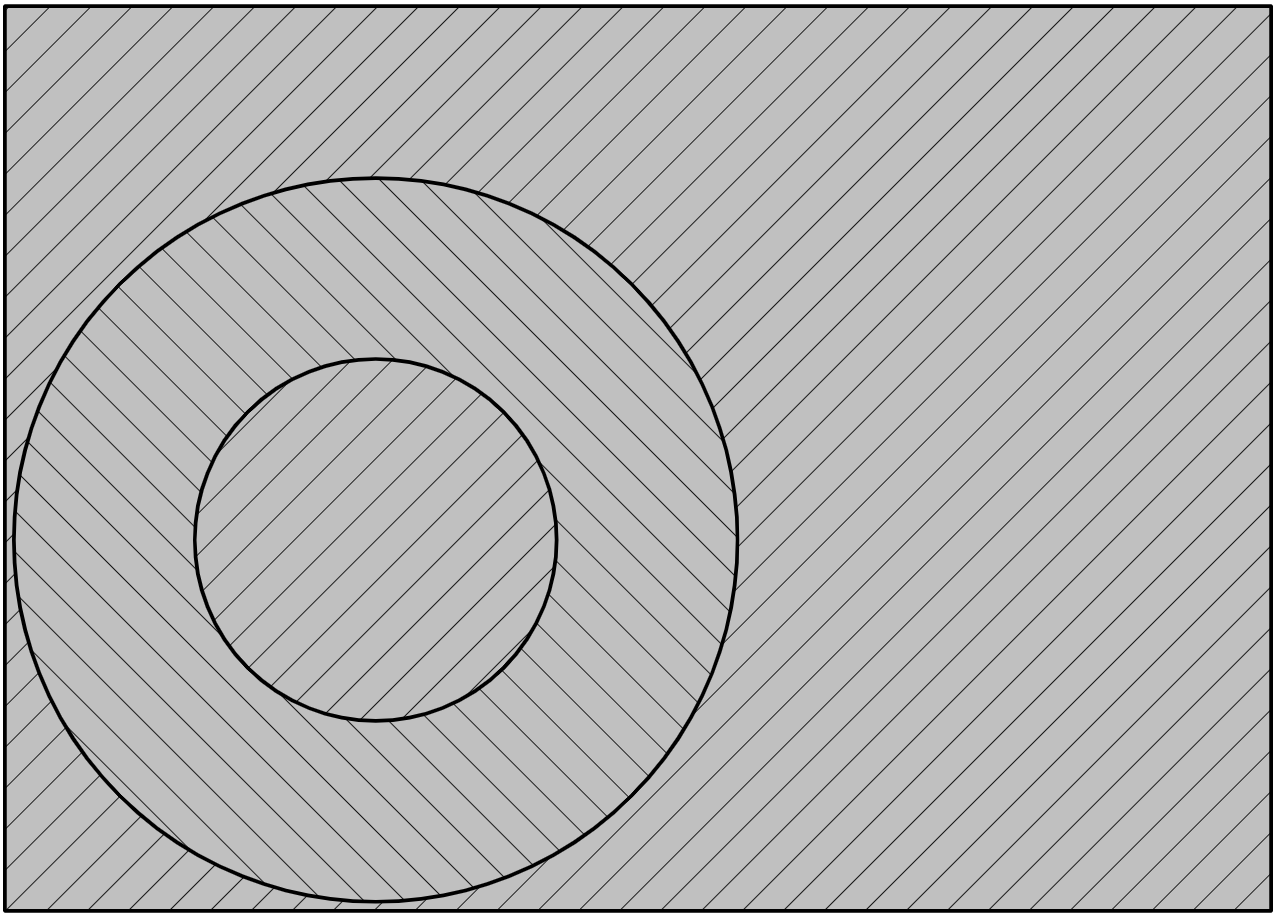
\includegraphics[width=0.61\textwidth]{nesting.png}
  \caption{Визуализация раскроя из Листинга~\ref{lst:dbs}}
  \label{fig:nesting}
\end{figure}

В ходе диссертационной работы
была разработан пакет утилит
\autocite{bi:dbs2json},
обеспечивающих конвертацию между
различными форматами файлов
(включая DBS, JSON, YAML, DXF и SVG для визуализации).
Для визуализации решения задачи PCGTSP
(на основе комбинации информации,
полученной из нескольких источников),
была разработана специализированная утилита,
первоначально в форме утилиты командной строки,
но позднее преобразованная
для удобства использования в
Single Page Application
(SPA)
и доступная по адресу
\url{https://ukoloff.github.io/j2pcgtsp/}.
Пример созданного ею изображения
приведён на рис.~\ref{fig:pcgtsp.svg}.

\begin{figure}
  \centering
  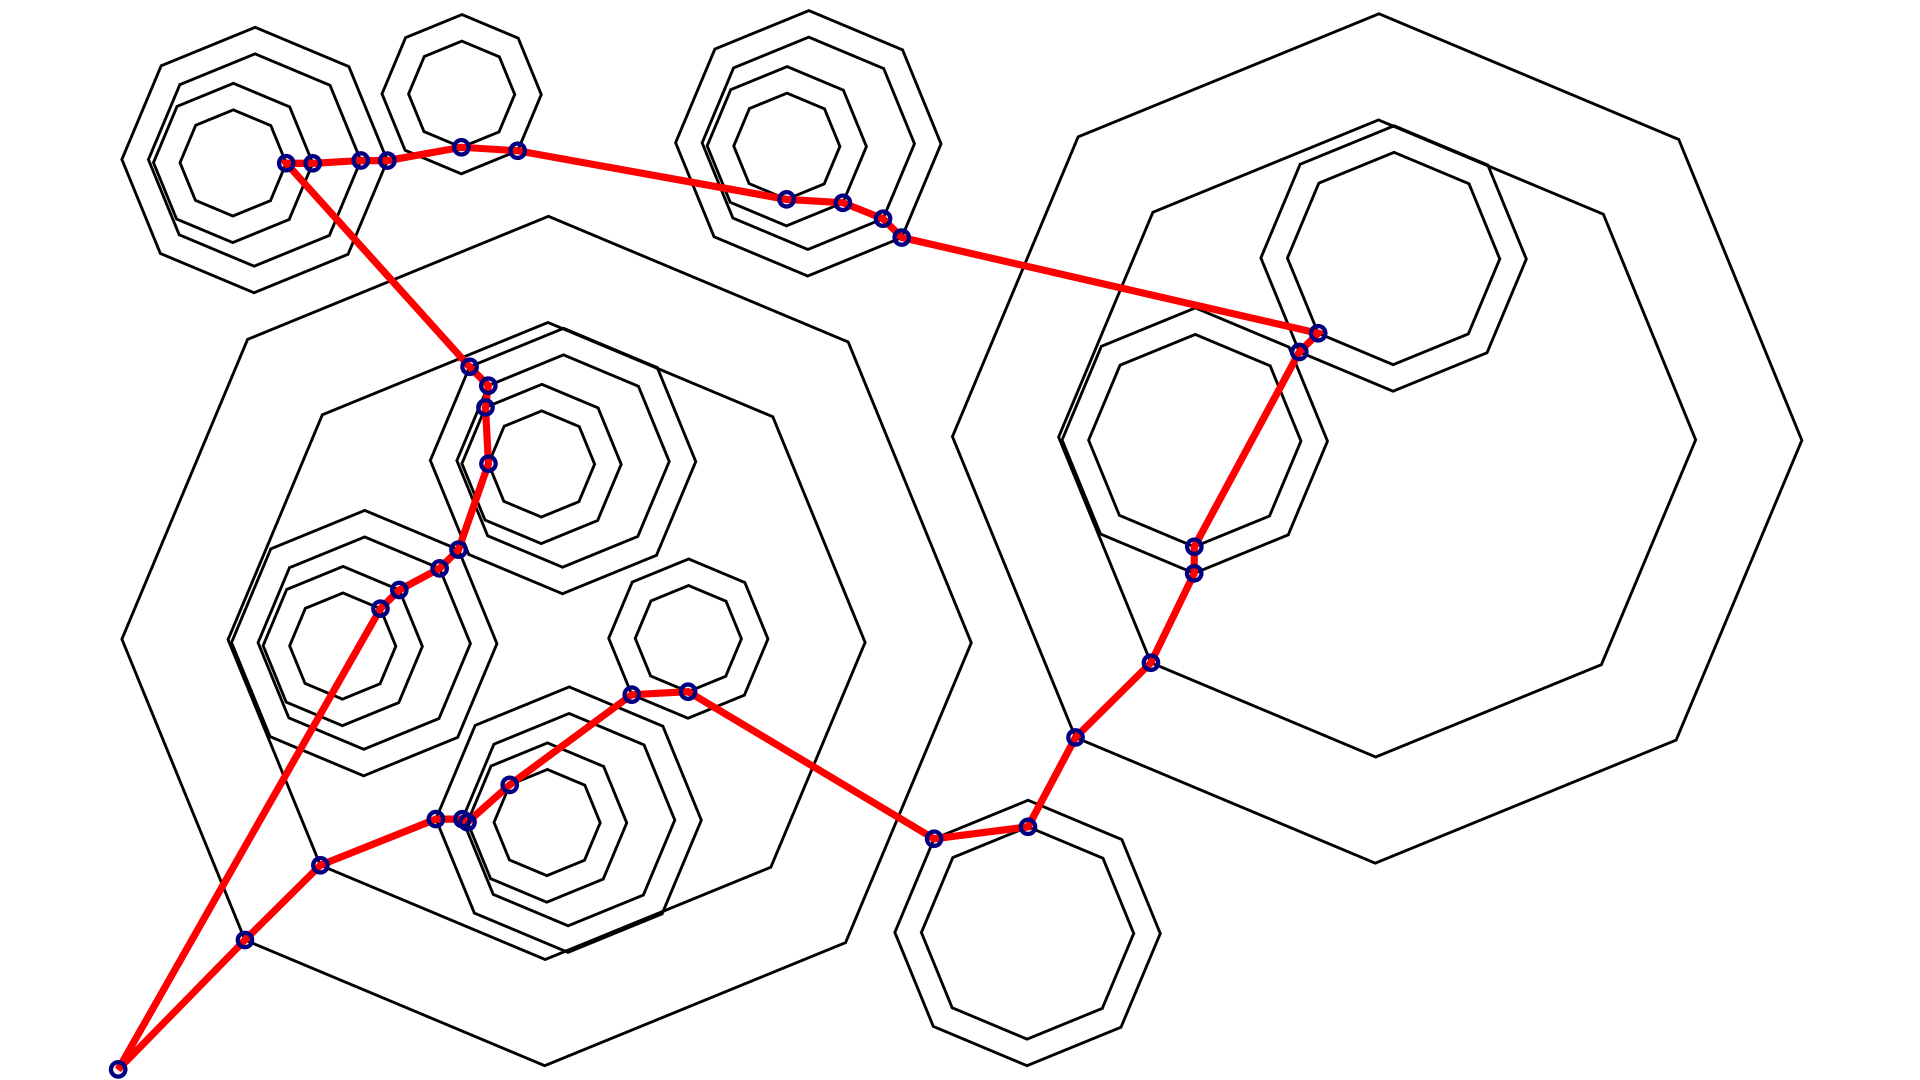
\includegraphics[width=0.95\textwidth]{34.png}
  \caption{Пример визуализации решения задачи PCGTSP}
  \label{fig:pcgtsp.svg}
\end{figure}


В {\bf заключении}
сформулированы основные научные и практические результаты
диссертационной работы.

В {\bf приложениях}
приведены
описание формата файла DBS
и JSON-схемы разработанных
в ходе работы форматов файлов.

